% Figure 25. A nonalgebraic Moishezon manifold (printed page 444).
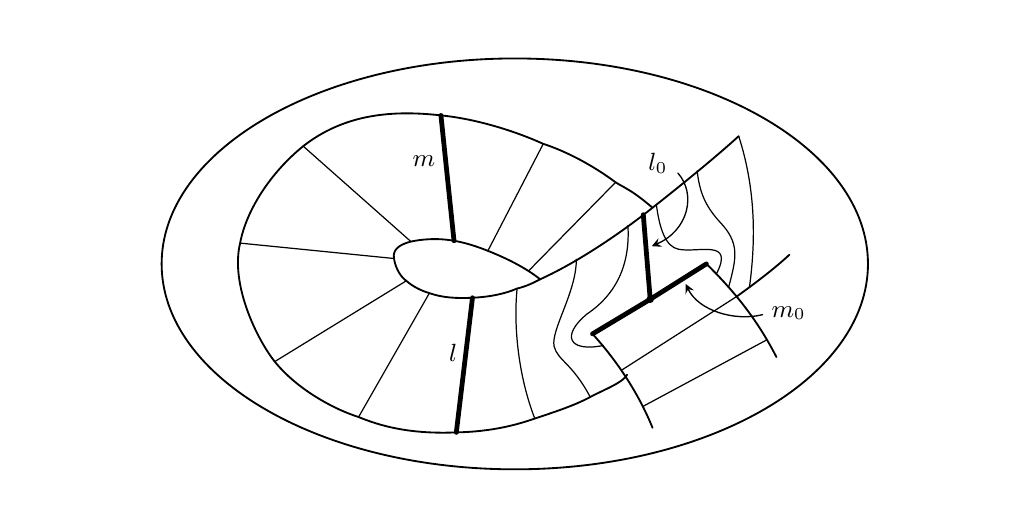
\begin{tikzpicture}[
    x=.277bp, y=-.277bp, line cap=round, line join=round, >=stealth,
    edge/.style={line width=.66bp},
    ruling/.style={line width=.44bp},
    fiber/.style={line width=1.72bp},
    leader/.style={->,line width=.48bp},
    every node/.style={font=\small,inner sep=0pt}
  ]
  \path[use as bounding box] (-162.1,-28) rectangle (1097.828,556.116);
  \draw[edge] (471,279) ellipse[x radius=459,y radius=267];

  \coordinate (join) at (504,299);
  \coordinate (upper-m) at (375,86);
  \coordinate (lower-m) at (392,249);
  \coordinate (upper-l) at (416,323);
  \coordinate (lower-l) at (395,498);
  \coordinate (double-point) at (647,325);
  \coordinate (rim-start) at (650,206);

  % The outer rim of the ruled band and the edge of the central opening.
  \draw[edge] (rim-start)
    .. controls (623,183) and (615,181) .. (602,173)
    .. controls (574,152) and (539,133) .. (508,123)
    .. controls (466,104) and (416,90) .. (upper-m)
    .. controls (305,78) and (246,87) .. (196,126)
    .. controls (154,160) and (122,209) .. (114,252)
    .. controls (101,306) and (136,377) .. (159,406)
    .. controls (188,442) and (236,468) .. (268,478)
    .. controls (306,494) and (347,500) .. (lower-l)
    .. controls (442,497) and (474,488) .. (497,480)
    .. controls (521,472) and (549,463) .. (569,452)
    .. controls (588,442) and (612,433) .. (617,423);
  \draw[edge] (join)
    .. controls (485,284) and (461,272) .. (436,262)
    .. controls (421,256) and (405,251) .. (lower-m)
    .. controls (370,245) and (350,247) .. (336,250)
    .. controls (320,254) and (312,261) .. (314,272)
    .. controls (316,286) and (324,297) .. (330,301)
    .. controls (339,309) and (350,314) .. (360,317)
    .. controls (377,323) and (395,324) .. (upper-l)
    .. controls (438,322) and (458,318) .. (474,311)
    .. controls (487,308) and (496,303) .. (join)
    .. controls (561,273) and (620,230) .. (rim-start)
    .. controls (683,180) and (729,143) .. (762,113);

  \draw[ruling]
    (196,126) -- (336,250)
    (114,252) -- (314,272)
    (159,406) -- (330,301)
    (268,478) -- (360,317)
    (508,123) -- (436,262)
    (602,173) -- (489,288)
    (474,311) .. controls (469,361) and (476,426) .. (497,480);

  % The two strips meeting in the exceptional fibers.
  \draw[edge]
    (572,370) .. controls (602,403) and (631,445) .. (650,492)
    (720,279) .. controls (759,317) and (788,355) .. (811,400)
    (760,321) .. controls (785,303) and (811,283) .. (828,267);
  \draw[ruling]
    (610,417) -- (760,321)
    (638,464) -- (798,378)
    (551,273) .. controls (551,316) and (518,364) .. (522,386)
      .. controls (527,405) and (545,407) .. (569,452)
    (618,229) .. controls (621,277) and (605,317) .. (565,344)
      .. controls (530,373) and (542,394) .. (586,385)
    (655,202) .. controls (659,233) and (667,257) .. (684,260)
      .. controls (709,265) and (757,246) .. (733,292)
    (708,158) .. controls (711,185) and (718,203) .. (737,224)
      .. controls (764,252) and (759,271) .. (749,309)
    (762,113) .. controls (783,178) and (785,243) .. (776,309);

  \draw[fiber]
    (upper-m) -- (lower-m)
    (upper-l) -- (lower-l)
    (638,215) -- (double-point)
    (572,370) -- (double-point) -- (720,279);
  \fill (double-point) circle[radius=1.35bp];

  \node at (353,145) {$m$};
  \node at (391,394) {$l$};
  \node at (657,148) {$l_0$};
  \node[anchor=west] at (804,343) {$m_0$};
  \draw[leader] (683,161)
    .. controls (707,188) and (697,235) .. (649,256);
  \draw[leader] (793,345)
    .. controls (757,354) and (710,340) .. (693,305);
\end{tikzpicture}
